
\documentclass[a4paper,12pt]{article}
\usepackage[margin=2cm]{geometry}

% Pacchetti utili di base
\usepackage[utf8]{inputenc}   % codifica dei caratteri
\usepackage[T1]{fontenc}      % font encoding
\usepackage[italian]{babel}   % lingua italiana
\usepackage{graphicx}         % immagini
\usepackage{hyperref}         % link cliccabili
\usepackage{amssymb} % oppure amsfonts
\usepackage{float}
\usepackage{amsmath}

% Informazioni sul documento
\title{Ingegneria del Software}
\author{Nicolò Giuliani}
\date{}


\begin{document}

\maketitle
\tableofcontents   % <-- genera automaticamente la pagina dell'indice
\newpage

\section{Introduzione}
La base del software engineering è la progettazione e lo sviluppo di software di alta qualità, affidabile e manutenibile. Questo documento esplora i principi fondamentali dell'ingegneria del software, le metodologie di sviluppo, e le best practice per garantire il successo dei progetti software.
\begin{figure}[H]
    \centering
    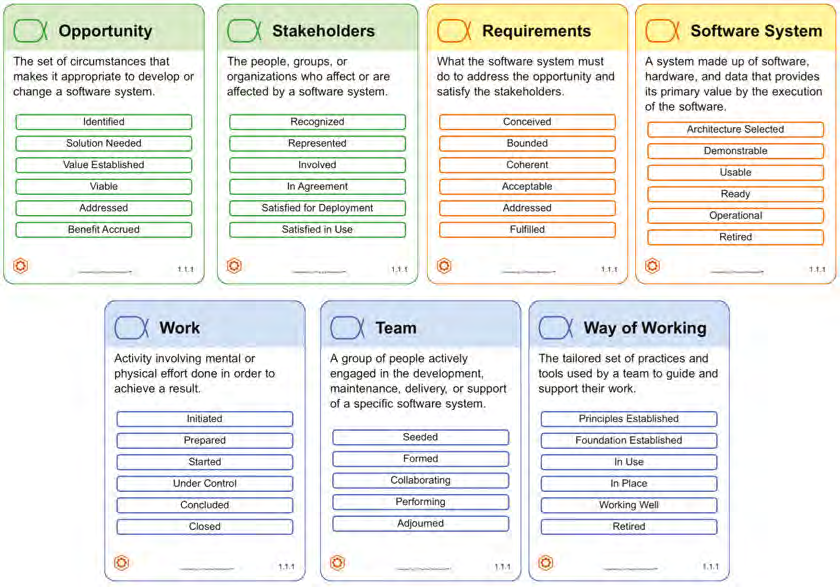
\includegraphics[width=0.9\textwidth]{img/Alpha Cards.png}
\end{figure}

\end{document}
